\subsubsection{Adapted SAGAT}
\label{subsubsec:results_adapted_sagat_1}

In this subsection, the SAGAT questionnaire is analyzed. Its result may give an idea of the mental map the participant is drawing. For each question a participant could score 1 point or a fraction of it. The total score of each blind participant is presented on the Table \ref{tab:sagat_table_blind} and they are plotted in the Figures \ref{fig:barplot_sagat_avg_5_scene_blind}, where it is visually noticeable that the performance better the second time they visit the room. 


\begin{table}[!htb]
\centering
\caption{SAGAT global score felled by the blinded participants.}
\label{tab:sagat_table_blind}
\begin{tabular}{llrrrrr}
\toprule
     &        &   Base &  Audio & \begin{tabular}[c]{@{}l@{}}Haptic\\ Belt\end{tabular} & \begin{tabular}[c]{@{}l@{}}Virtual\\ Cane\end{tabular} & Mixture \\
Participant & Round &        &        &                                                       &                                                        &         \\
\midrule
001C & First &   6.25 &   5.50 &                                                  5.33 &                                                   5.83 &   3.500 \\
     & Return &   6.25 &   6.50 &                                                  8.50 &                                                   5.50 &   5.500 \\
002C & First &   6.75 &   4.50 &                                                  3.99 &                                                   4.50 &   6.250 \\
     & Return &   5.25 &   5.00 &                                                  4.00 &                                                   6.50 &   8.500 \\
003C & First &   7.25 &   7.50 &                                                  7.49 &                                                   4.66 &   9.000 \\
     & Return &  10.00 &  10.00 &                                                  8.50 &                                                   9.00 &   9.000 \\
004C & First &   7.50 &   6.00 &                                                  7.66 &                                                   4.99 &   6.500 \\
     & Return &   9.00 &   6.00 &                                                  9.25 &                                                   7.25 &   9.000 \\
\bottomrule
\end{tabular}
\end{table}



\begin{figure}[!htb]
    \centering
    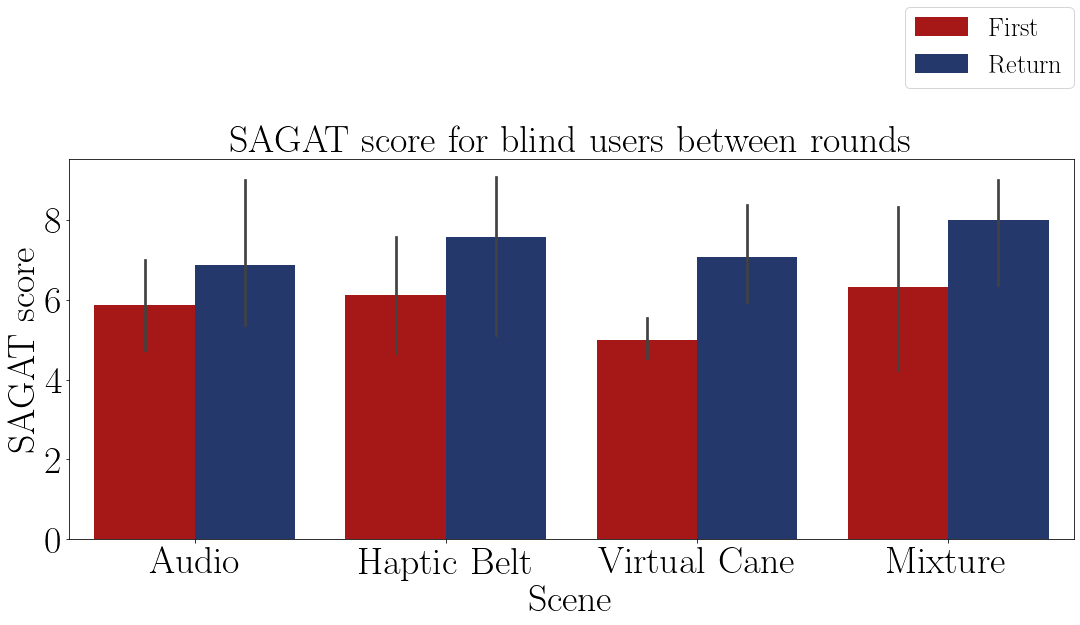
\includegraphics[width = 0.8\linewidth]{Resultados/Sagat/Figuras/png/barplot_sagat_avg_5_scene_blind.png}
    \caption{Barplot of the average SAGAT score of the blind participants on each method.}
    \label{fig:barplot_sagat_avg_5_scene_blind}
\end{figure}

The boxplot in the Figure \ref{fig:boxplot_sagat_blind_scene} shows that there are two groups of scores one with the “Base”, “Haptic Belt” and the “Mixture” methods, and the second group with the “Audio” and the “Virtual Cane” methods. The first group scored higher than the second one. The Figure \ref{fig:boxplot_sagat_blind_rounds} shows a noticible difference between the scores when grouped by their corresponding round.

\begin{figure}[!htb]
    \centering
    \begin{minipage}{0.45\textwidth}
        \centering
        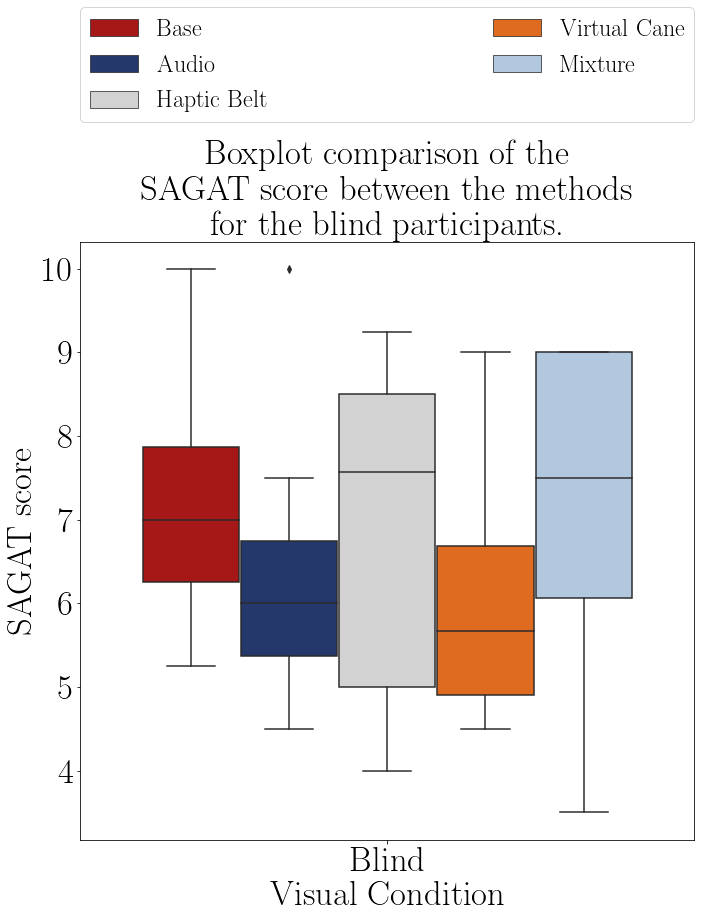
\includegraphics[width = 0.8\linewidth]{Resultados/Sagat/Figuras/png/boxplot_sagat_blind_scene.png}
        \caption{Boxplot of the SAGAT score of the blind participants grouped by method.}
        \label{fig:boxplot_sagat_blind_scene}
    \end{minipage}
    \begin{minipage}{0.45\textwidth}
        \centering
        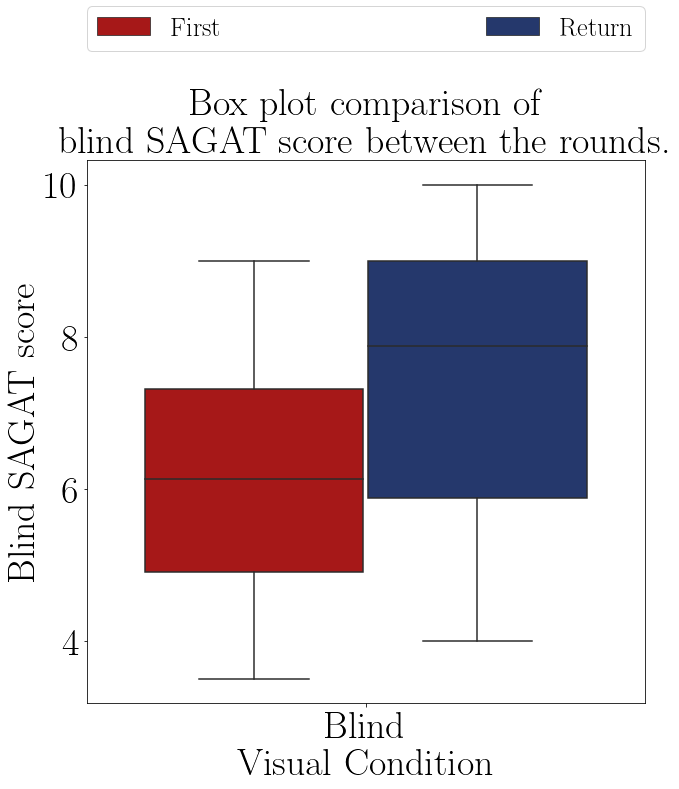
\includegraphics[width = 0.8\linewidth]{Resultados/Sagat/Figuras/png/boxplot_sagat_blind_rounds.png}
        \caption{Boxplot of the SAGAT score of the blind participants grouped by round.}
        \label{fig:boxplot_sagat_blind_rounds}
    \end{minipage}
\end{figure}

The Table \ref{tab:sagat_average_group_blind} shows the average SAGAT score in the “blind” sample and is possible to notice how the average score by the “blind” sample was lower during the “Audio” and the “Base” methods.


\begin{table}[!htb]
\centering
\caption{SAGAT score average grouped by participant and visual condition}
\label{tab:sagat_average_group_blind}
\begin{tabular}{lrrrrrr}
\toprule
{} &  Base & Audio & \begin{tabular}[c]{@{}l@{}}Haptic\\ Belt\end{tabular} & \begin{tabular}[c]{@{}l@{}}Virtual\\ Cane\end{tabular} &  Mixture \\
Visual Condition &       &       &                                                       &                                                        &          \\
\midrule
Blind            &  7.28 &  6.38 &                                                  6.84 &                                                   6.03 &    7.156 \\
\bottomrule
\end{tabular}
\end{table}




The Figures \ref{fig:qqplot_sagat_avg_two_way_blind} and \ref{fig:residplot_sagat_avg_two_way_blind} shows the distribution and variance of the Table \ref{tab:sagat_table_blind}. These Figures shows that the data are normally distributed and that the methods have a similar variance.
The Table \ref{tab:blocanova_sagat_avg_two_way_blind} shows the Anova test p-value of the SAGAT score of the "blind" sample. The round's p-values indicates that some have influence on the SAGAT score. Meaning that the participants did learn information about the room between the "First" and "Return" round. The method and the interaction between it and the round has no influence on the SAGAT score.


\begin{table}[!htb]
\centering
\caption{Anova p-value for the SAGAT score on each method for blinded users.}
\label{tab:blocanova_sagat_avg_two_way_blind}
\begin{tabular}{lrrrrr}
\toprule
               Source &  Squared sum &  DOF & Squared average &      F & \begin{tabular}[c]{@{}l@{}}P-Value \\ $(F_{0} > F)$\end{tabular} \\
\midrule
Participants (Blocks) &       48.231 &    3 &          16.077 &  9.731 &                                                                  \\
         \    Methods &        8.922 &    4 &           2.230 &  1.350 &                                                            0.277 \\
          \    Rounds &       18.975 &    1 &          18.975 & 11.485 &                                                          0.002** \\
     \    Interaction &        2.391 &    4 &           0.598 &  0.362 &                                                            0.834 \\
   Experimental Error &       44.608 &   27 &           1.652 &        &                                                                  \\
                Total &      123.127 &   39 &                 &        &                                                                  \\
\bottomrule
\end{tabular}
\end{table}



\begin{figure}[!htb]
    \centering
    \begin{minipage}{0.45\textwidth}
        \centering
        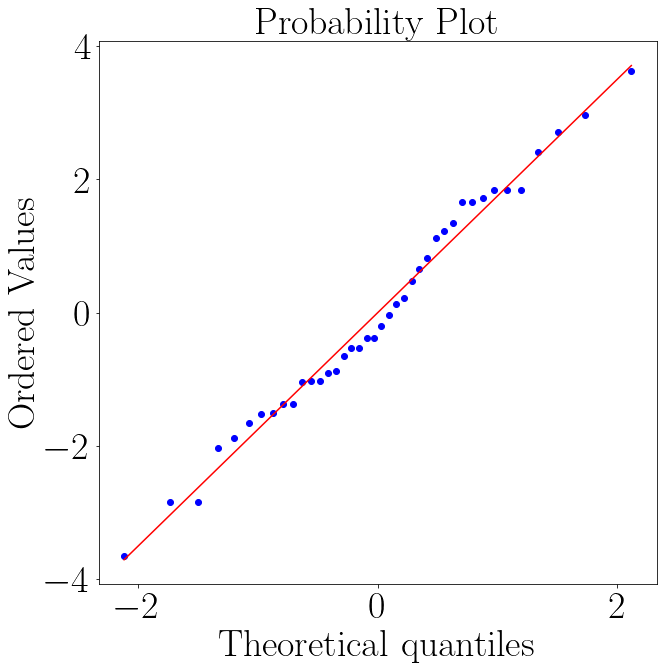
\includegraphics[width = 0.8\linewidth]{Resultados/Sagat/Figuras/png/qqplot_sagat_avg_two_way_blind.png}
        \caption{QQ plot of the SAGAT score of the blind participants on each method.}
        \label{fig:qqplot_sagat_avg_two_way_blind}
    \end{minipage}
    \begin{minipage}{0.45\textwidth}
        \centering
        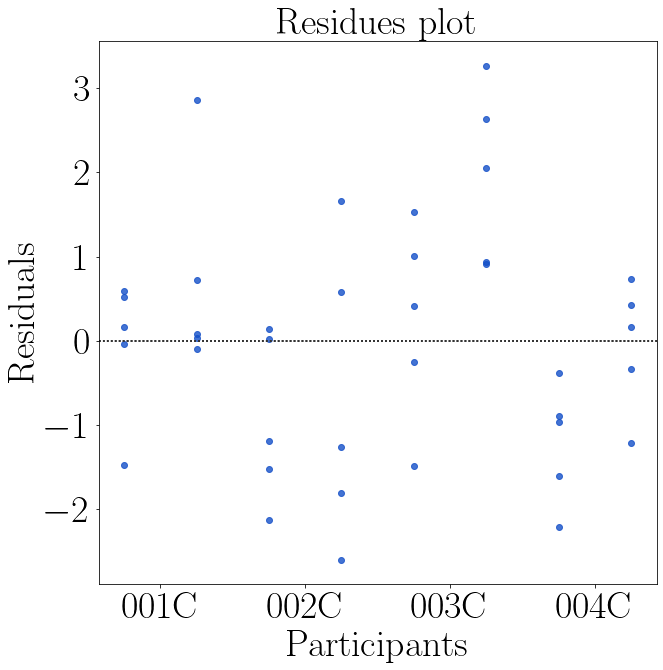
\includegraphics[width = 0.8\linewidth]{Resultados/Sagat/Figuras/png/residplot_sagat_avg_two_way_blind.png}
        \caption{Residual plot of the SAGAT score the blind participants on each method.}
        \label{fig:residplot_sagat_avg_two_way_blind}
    \end{minipage}
\end{figure}


%The Table \ref{tab:lsd_sagat_avg_two_way} presents the conclusion of a pairwise Fisher LSD test of the blind NASA-TLX score between all the guidance methods. The results show that only the "Audio" has a similar NASA-TLX score as the "Base" method, as it was also posible to notice at Figure \ref{fig:boxplot_sagat_blind_scene}.

%\input{Resultados/Sagat/Tabelas/lsd_sagat_avg_two_way}

The Table \ref{tab:sagat_var_group_blind} shows the average of the SAGAT score variation between the rounds. This table shows that the variation from the "Base" and the "Audio" was the lowest variation and the highest variation was the "Virtual Cane".


\begin{table}[!htb]
\centering
\caption{Adapted Sagat global score variation grouped by participant and visual Condition}
\label{tab:sagat_var_group_blind}
\begin{tabular}{lrrrrrr}
\toprule
{} &  Base &  Audio & \begin{tabular}[c]{@{}l@{}}Haptic\\ Belt\end{tabular} & \begin{tabular}[c]{@{}l@{}}Virtual\\ Cane\end{tabular} & Mixture \\
Visual Condition &       &        &                                                       &                                                        &         \\
\midrule
Blind            &  8.93 &  15.66 &                                                 23.49 &                                                  44.30 &   32.90 \\
\bottomrule
\end{tabular}
\end{table}



The Figures \ref{fig:qqplot_sagat_var_blind} and \ref{fig:residplot_sagat_var_blind} shows the distribution and variance of the SAGAT score variation of the Table \ref{tab:sagat_table_blind}. These Figures shows that the data are normally distributed and that the methods have a similar variance.
The Table \ref{tab:blocanova_sagat_var_blind} shows the Anova test p-value of the SAGAT score of the "blind" sample between the guidance methods. The p-value indicates that there are no difference between the variation in any method. 


\begin{table}[!htb]
\centering
\caption{Anova p-value for the SAGAT score variation on each method for blinded users.}
\label{tab:blocanova_sagat_var_blind}
\begin{tabular}{lrrrrr}
\toprule
               Source &  Squared sum &  DOF & Squared average &     F & \begin{tabular}[c]{@{}l@{}}P-Value \\ $(F_{0} > F)$\end{tabular} \\
\midrule
Participants (blocks) &     1176.902 &    3 &         782.885 & 0.473 &                                                                  \\
               Method &     3131.542 &    4 &         392.301 & 0.944 &                                                            0.472 \\
   Experimental error &     9956.458 &   12 &         829.705 &       &                                                                  \\
                Total &    14264.902 &   19 &                 &       &                                                                  \\
\bottomrule
\end{tabular}
\end{table}



\begin{figure}[!htb]
    \centering
    \begin{minipage}{0.45\textwidth}
        \centering
        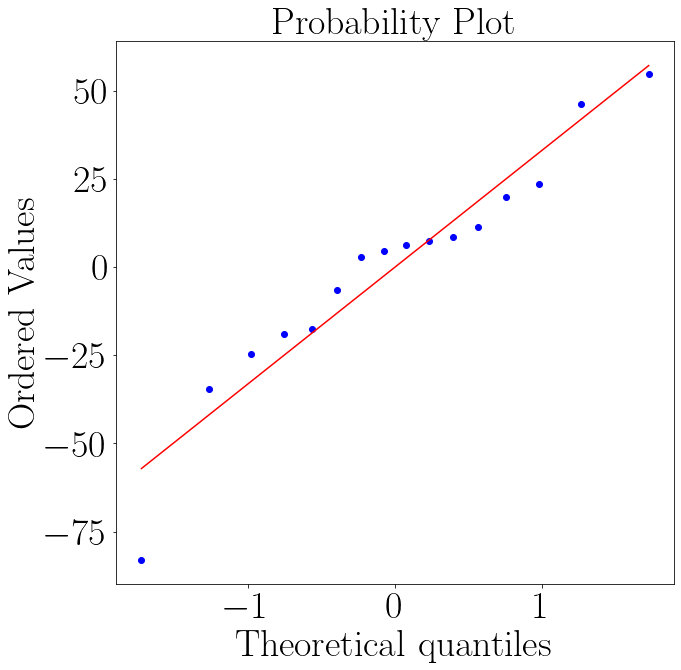
\includegraphics[width = 0.8\linewidth]{Resultados/Sagat/Figuras/png/qqplot_sagat_var_sight.png}
        \caption{QQ plot of the SAGAT score variation of the blind participants on each method.}
        \label{fig:qqplot_sagat_var_blind}
    \end{minipage}
    \begin{minipage}{0.45\textwidth}
        \centering
        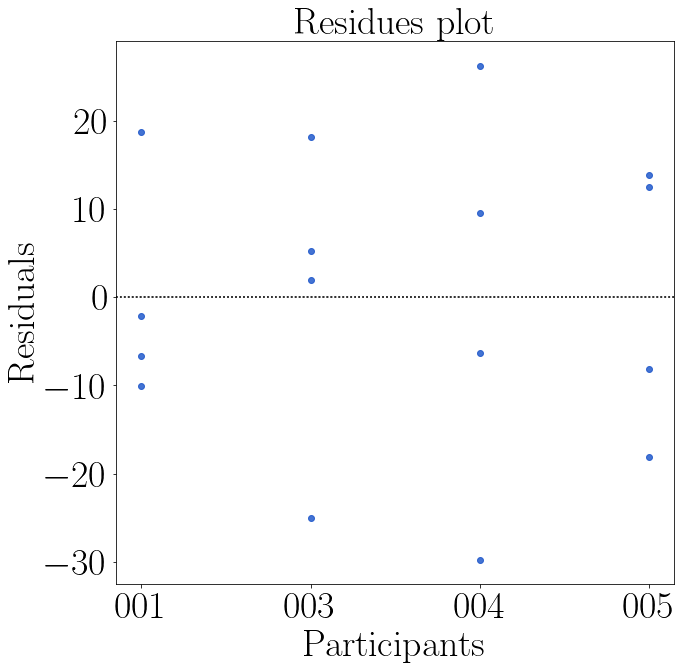
\includegraphics[width = 0.8\linewidth]{Resultados/Sagat/Figuras/png/residplot_sagat_var_sight.png}
        \caption{Residual plot of the SAGAT score variation of the blind participants on each method.}
        \label{fig:residplot_sagat_var_blind}
    \end{minipage}
\end{figure}

%The Table \ref{tab:lsdbloc_nasa_var} presents the conclusion of a pairwise Fisher LSD test of the blind NASA-TLX score between all the guidance methods. The results show that all methods have similar variations.

%
\begin{table}[!htb]
\centering
\caption{Cross validation p-value for the NASA-TLX score variation on each method for blinded users.}
\label{tab:lsdbloc_nasa_var}
\begin{tabular}{rclr}
\toprule
      \multicolumn{3}{c}{Method} &                                       Analysis \\
\midrule
              Base & $X$ & Audio &           $H_1 : \mu_{Base} \ne \mu_{Audio}**$ \\
        Base & $X$ & Haptic Belt &         $H_0 : \mu_{Base} = \mu_{Haptic Belt}$ \\
       Base & $X$ & Virtual Cane &    $H_1 : \mu_{Base} \ne \mu_{Virtual Cane}**$ \\
            Base & $X$ & Mixture &             $H_0 : \mu_{Base} = \mu_{Mixture}$ \\
       Audio & $X$ & Haptic Belt &    $H_1 : \mu_{Audio} \ne \mu_{Haptic Belt}**$ \\
      Audio & $X$ & Virtual Cane &   $H_1 : \mu_{Audio} \ne \mu_{Virtual Cane}**$ \\
           Audio & $X$ & Mixture &            $H_0 : \mu_{Audio} = \mu_{Mixture}$ \\
Haptic Belt & $X$ & Virtual Cane & $H_0 : \mu_{Haptic Belt} = \mu_{Virtual Cane}$ \\
     Haptic Belt & $X$ & Mixture &  $H_1 : \mu_{Haptic Belt} \ne \mu_{Mixture}**$ \\
    Virtual Cane & $X$ & Mixture & $H_1 : \mu_{Virtual Cane} \ne \mu_{Mixture}**$ \\
\bottomrule
\end{tabular}
\end{table}



To close up, according to the ANOVA test at Table \ref{tab:blocanova_sagat_avg_two_way_blind} the methods caused no reaction on the SAGAT score, but the rounds did. That means that the participants were able in all methods to learn a little about their environment and that learning impacted their environmental perception in the next round. The fact that the test has not found any influence of the methods on the SAGAT score may be because of the small sample size, since it is posible to notice a difference between the methods at Figure \ref{fig:boxplot_sagat_blind_scene}. Also the interaction between method and round caused no influence in the Sagat score. According to the ANOVA test at Table \ref{tab:blocanova_sagat_var_blind}, the methods did not influenced the SAGAT score.

\FloatBarrier